\begin{figure}[h!]
\centering
%\resizebox{columnwidth}{2cm}{
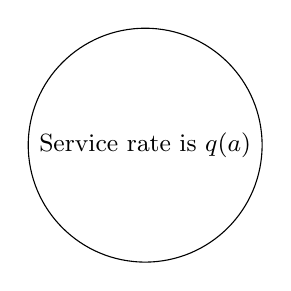
\begin{tikzpicture}[domain=0:7.7,scale=0.7,font=\small,axis/.style={very thick, ->, >=stealth'}]
\node[draw, circle](one) at (5,1) {Service rate is $q(a)$};
%\draw[->, =>latex](one) edge[bend left=42.5](two);
%\node [above=1.1cm]at (2.8,1.2) {${p_{a_n}(s,s')}$};
%\node [right] at(0,0){$g_{a_n}(s_n)$};
\end{tikzpicture}
%}
\caption{Single queue with controlled service.}
\label{schematic}
\end{figure}
